%\documentclass[aspectratio=43]{beamer}
%\documentclass[aspectratio=169]{beamer}
\documentclass[aspectratio=1610,12pt]{beamer}
\usepackage[utf8]{inputenc}
\usepackage[T1]{fontenc}
\usepackage{lmodern}

\usepackage[ngerman]{babel}
%\usepackage[ngerman]{babel} %use this for German presentations
\usepackage{booktabs} % fancy tables
\usepackage{tabulary} % tables with auto column length
\usepackage{hyperref}

\usetheme{imise2}
\author{Konrad Höffner}
\date{Leipzig, 15.Mai 2020}
\title{HITO}
\subtitle{Werkzeuge für die Navigation durch}
\def\address{Härtelstraße 16-18, 04107 Leipzig, Raum 227}
\def\email{konrad.hoeffner@imise.uni-leipzig.de}
\def\telephone{+49 341 97 16322}

\begin{document}
\begin{frame}
\titlepage
\end{frame}

\begin{frame}{Überblick}
\begin{itemize}
\item first
\item second
\end{itemize}
\end{frame}

\begin{frame}{Hito Bahmni}
  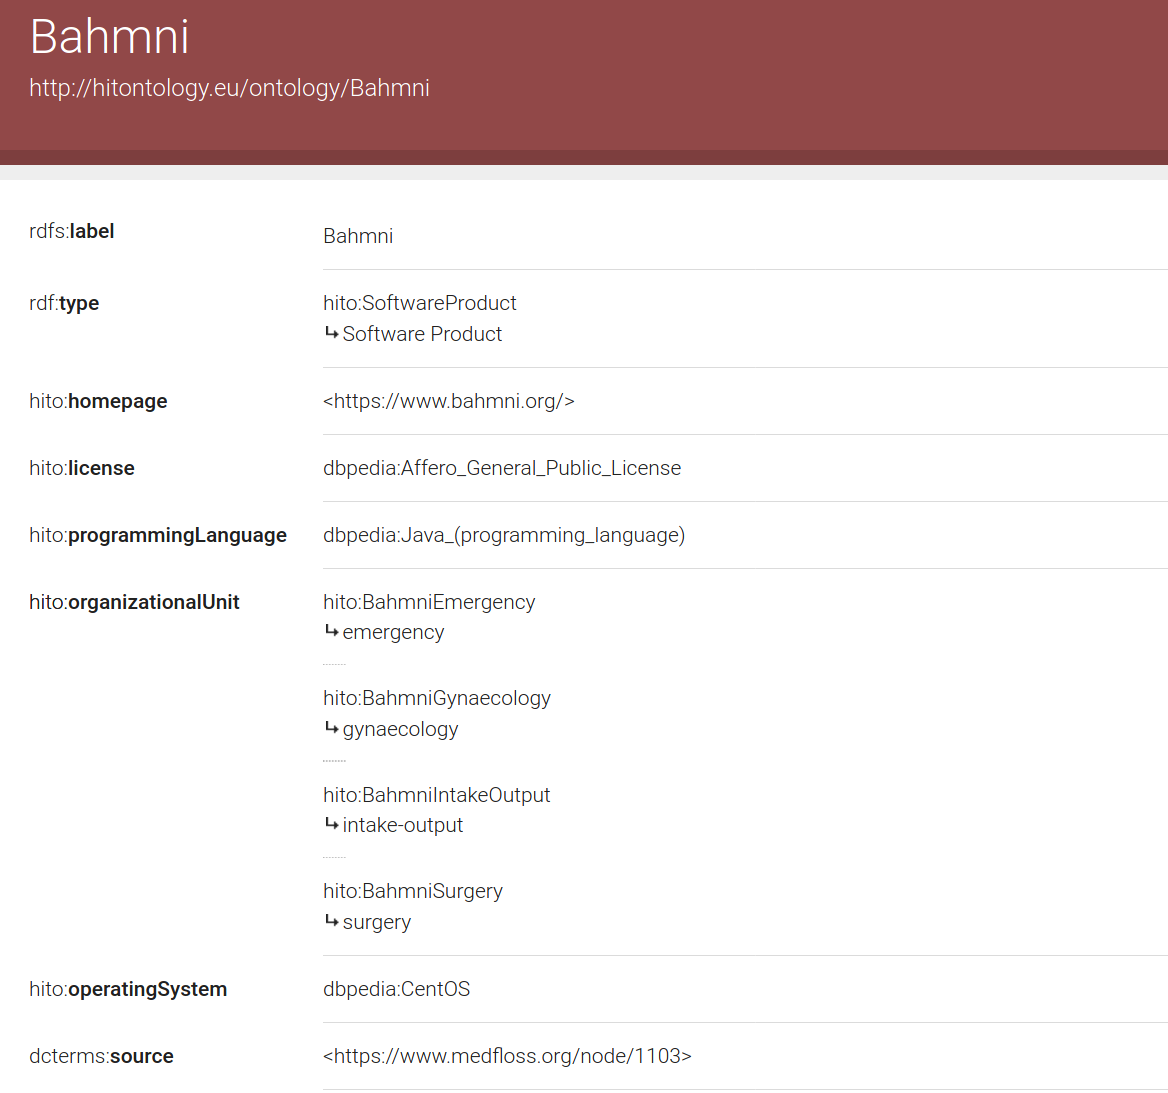
\includegraphics[width=\textwidth]{img/hito-bahmni.png}
\end{frame}

\begin{frame}{Medfloss Bahmni}
  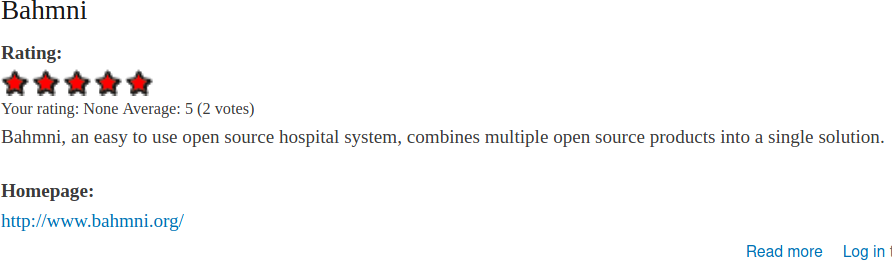
\includegraphics[width=\textwidth]{img/medfloss-bahmni.png}
\end{frame}

\begin{frame}{Medfloss Bahmni Link}
  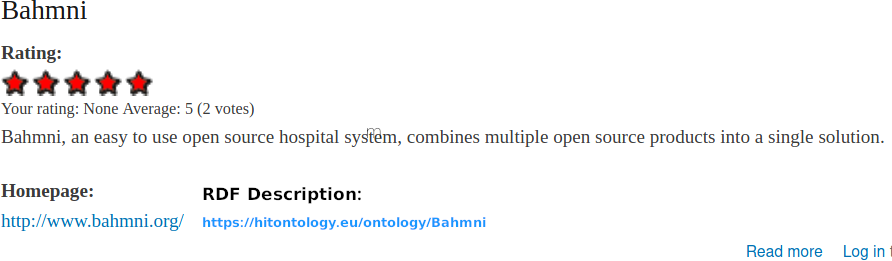
\includegraphics[width=\textwidth]{img/medfloss-bahmni-link.png}
\end{frame}


\end{document}
